%%%%%%%%%%%%%%%%%%%%%%%%%%%%%%%%%%%%%%%%%%%%%%%%%%%%%%%%%%%%%%%%%%%%%
% Template for Master work
%%%%%%%%%%%%%%%%%%%%%%%%%%%%%%%%%%%%%%%%%%%%%%%%%%%%%%%%%%%%%%%%%%%%%%
\documentclass[12pt,a4paper,notitlepage,colorinlistoftodos]{article} 
% can add 'draft' to unload figures
%===================================================================%
%\begin{} Hiding most package loading and precisions
%===================================================================%
% set up file for new commands and main packages :
\providecommand{\main}{.}  % *Modification: define file location
\usepackage{\main/.temp/setup}
%%%%%%%%%%%%%%%%%%%%%%%%%%%%%%%%%%%%%%%%%%%%%%%%%%%%%%%%%%%%%%%%%%%%%%
% Page de garde
%%%%%%%%%%%%%%%%%%%%%%%%%%%%%%%%%%%%%%%%%%%%%%%%%%%%%%%%%%%%%%%%%%%%%%
% Informations :
\logolab{fig/labo.jpg}
\title{Title : An example report in latex for my master degree in Grenoble.}
\author{Maxime Jaunatre $^1$}
\souten{mardi 2 juin 2020}
\tutor{François Munoz}
\labo{LECA}
\team{Bouclés}
\labadr{CIRAD, TA A51/PS2, Boulevard de la Lironde,\\ 34398 Montpellier cedex 5}
\pict{fig/Primula_hirsuta_Grand_Chat_longistyle.JPG}
\credpict{Image : \textit{Primula hirsuta}, Florian Boucher}
\email{maxime.jaunatre@etu.univ-grenoble-alpes.fr}
%%%%%%%%%%%%%%%%%%%%%%%%%%%%%%%%%%%%%%%%%%%%%%%%%%%%%%%%%%%%%%%%%%%%%%
% Quick set up
%%%%%%%%%%%%%%%%%%%%%%%%%%%%%%%%%%%%%%%%%%%%%%%%%%%%%%%%%%%%%%%%%%%%%%
\setboolean{notes}{true} % display notes done with the todonotes package
\setboolean{terminal}{false} % compile document with dark colour to help your pretty eyes
\setboolean{counter}{true} % add a word count at the end of the document
\setboolean{bib_basic}{true} % bib_basic use authordate format, with false you can provide a .bst file 
\usepackage{\main/.temp/subfile_setup}
%%%%%%%%%%%%%%%%%%%%%%%%%%%%%%%%%%%%%%%%%%%%%%%%%%%%%%%%%%%%%%%%%%%%%
% language
\usepackage[french]{babel} % or 'english'
% Don't forget to change the table of content
\hyphenation{geo-graphique} % add '\-' to create custom hypernation if a word is difficult to cut or :
%% texmaker change language for auto correction
%%fr folder : /usr/share/myspell/dicts/fr_FR.dic
%%uk folder : /usr/share/hunspell/en_GB.dic
%%%%%%%%%%%%%%%%%%%%%%%%%%%%%%%%%%%%%%%%%%%%%%%%%%%%%%%%%%%%%%%%%%%%%
% all other packages and functions
\usepackage{\main/.temp/packages}
%%%%%%%%%%%%%%%%%%%%%%%%%%%%%%%%%%%%%%%%%%%%%%%%%%%%%%%%%%%%%%%%%%%%%
% Custom document commands
\renewcommand*\contentsname{Table des matières}
%\newcommand{\defi}[2]{\textbf{#1: }{#2}}
\newcommand{\defi}[2]{\textbf{#1: }{#2}}
\newcommand{\imp}[1][this!]{ {\todo[inline,color=red]{\textbf{Check: #1}} } }


\newcommand{\clade}[1]{clade `#1'}
%%%%%%%%%%%%%%%%%%%%%%%%%%%%%%%%%%%%%%%%%%%%%%%%%%%%%%%%%%%%%%%%%%%%%%
%===================================================================%
%\end{}
%===================================================================%
%%%%%%%%%%%%%%%%%%%%%%%%%%%%%%%%%%%%%%%%%%%%%%%%%%%%%%%%%%%%%%%%%%%%%%
\begin{document}
\def\biblio{} \def\sub_title{} \def\setup{}
%%%%%%%%%%%%%%%%%%%%%%%%%%%%%%%%%%%%%%%%%%%%%%%%%%%%%%%%%%%%%%%%%%%%%%
% Title
%%%%%%%%%%%%%%%%%%%%%%%%%%%%%%%%%%%%%%%%%%%%%%%%%%%%%%%%%%%%%%%%%%%%%%
\subfile{.temp/frontpage}
%%%%%%%%%%%%%%%%%%%%%%%%%%%%%%%%%%%%%%%%%%%%%%%%%%%%%%%%%%%%%%%%%%%%%%
% Abstract
% ignore todo in wordcount !
%TC:macro \todo [0]
%%%%%%%%%%%%%%%%%%%%%%%%%%%%%%%%%%%%%%%%%%%%%%%%%%%%%%%%%%%%%%%%%%%%%%
\newpage
\begin{abstract}

\lipsum[1]
\imp

\begin{center}
\textbf{Abstract}
\end{center}

\lipsum[1]
\imp

\end{abstract}
\todo[inline,color=gray]{note that this is an example of abstract in 2 language}

%%%%%%%%%%%%%%%%%%%%%%%%%%%%%%%%%%%%%%%%%%%%%%%%%%%%%%%%%%%%%%%%%%%%%%
% Table des matières
%%%%%%%%%%%%%%%%%%%%%%%%%%%%%%%%%%%%%%%%%%%%%%%%%%%%%%%%%%%%%%%%%%%%%%
\newpage
\tableofcontents
\thispagestyle{empty}
\todo[inline,color=gray]{note that this page style is 'empty' and have no page number for example}

%%%%%%%%%%%%%%%%%%%%%%%%%%%%%%%%%%%%%%%%%%%%%%%%%%%%%%%%%%%%%%%%%%%%%%
% Todo list
%%%%%%%%%%%%%%%%%%%%%%%%%%%%%%%%%%%%%%%%%%%%%%%%%%%%%%%%%%%%%%%%%%%%%%
\ifthenelse{\boolean{notes}}{
	\listoftodos
	\hrule\bigskip 
}{}
\todo[inline,color=gray]{note that this todo list will disappear if you set notes on false or comment it}
%%%%%%%%%%%%%%%%%%%%%%%%%%%%%%%%%%%%%%%%%%%%%%%%%%%%%%%%%%%%%%%%%%%%%%
% BODY
\newpage
%%%%%%%%%%%%%%%%%%%%%%%%%%%%%%%%%%%%%%%%%%%%%%%%%%%%%%%%%%%%%%%%%%%%%%


This document provide all the command I usually use for my reports. Gray notes are here to explain some stuff, while red ones are here to be a last line limit when I wrote my report too close to the deadline and misread colours. I defined a new todonotes juste for this, to help me manage my work. 

\imp[imp command]

\section{Basic commands}

Here is some memory about basic latex commands. Like putting some text in \textit{italic} for species names. Or \textbf{bold} for important parts. This is completed with a possibility to highlight with the \hl{hl} command. The colour is defined at the very beginning of the document, but another command allow to change with \hlc[red]{hlc[red]word}. Every colour is possible and you can define them by the xcolor package.

Below is an exemple of a list

\begin{itemize}
  \item Item A.
  \item Item B.
  \begin{enumerate}
  	\item sub part 1
  	\item sub part 2
  \end{enumerate}
  \item Item C
\end{itemize}

\section{To do notes}

To help in long work redaction, the todonotes package is loaded by default, allowing to set inline or marge todonotes \todo[color = gray]{marge}. Authors can be specified and the list of to do is loaded at the beginning of the document. Everything is explain in more detail inside this document \url{http://tug.ctan.org/macros/latex/contrib/todonotes/todonotes.pdf}

\todo[inline, color = gray]{inline}
\todo[inline, author = Gowachin, color = gray]{specifying the author of the todo comment}

\section{Maths}

Some packages are also loaded to allow maths equations to be displayed.

\begin{equation}
Y \in B;  B = {a,c,g,t}
\label{eq:11}
\end{equation}

\begin{equation}
\begin{cases}
prey_{t+1} = prey_{t} + prey_{t} \cdot r \cdot (1 - prey_{t} / K ) + int_{pred/prey} \cdot pred_{t} \\
pred_{t+1} = pred_{t} + pred_{t} \cdot r \cdot (1 - pred_{t} / K ) + int_{prey/pred} \cdot prey_{t}
\end{cases}
\label{eq:lotk}
\end{equation}
\textit{with : \textbf{r} the growth rate and \textbf{K} the capacity.} \\

\section{Captions}

Multiple captions are possible, like tables, figures and boxes, as display below. To show all the possibilities, there is \textbf{Lorem ipsum} text around. 

\begin{wrapfigure}{R}{3.10in}
\begin{wordbox}
 \\ \defi{Phylogeny}{Object resuming evolutionary relation between living beings by illustrating distance between them. Mostly represented as a phylogenetic tree.}\\
\defi{Community}{An assemblage of populations from different species, defined by a time and geographic scale restriction. This assemblage can also be represented by interactions between these populations.}\\
\end{wordbox}
%\vspace{-20pt}
\end{wrapfigure}

\lipsum[1-3]

\begin{figure}[h] %{R}{3.00in}
\begin{bluebox}{More complex null model, Pigot \textit{et al.} (2015) \\}

\textbf{Context: }To study the assembly processes of a community, ecologist compare metrics (in this example the Mean Nearest Taxon Distance) with randow draw species in the community. This null model is easily applicable but build assumption issues. For example, these null models don't take into account the historical aspect of community assembly.

\textbf{Results: }Authors found that their null models produce overdispersed community, by just taking into account historical aspect of colonisation and extinction in contrast with just random draw of species. Empirical data shown significantly  overdispersed species in the community but fail to reject this null model. 

Therefore, overdispertion could just arise from historical processes, independent from traits or biotic interactions. This new null model invite us to rethink more precedent result where overdispersion had been found.

%\begin{figure}
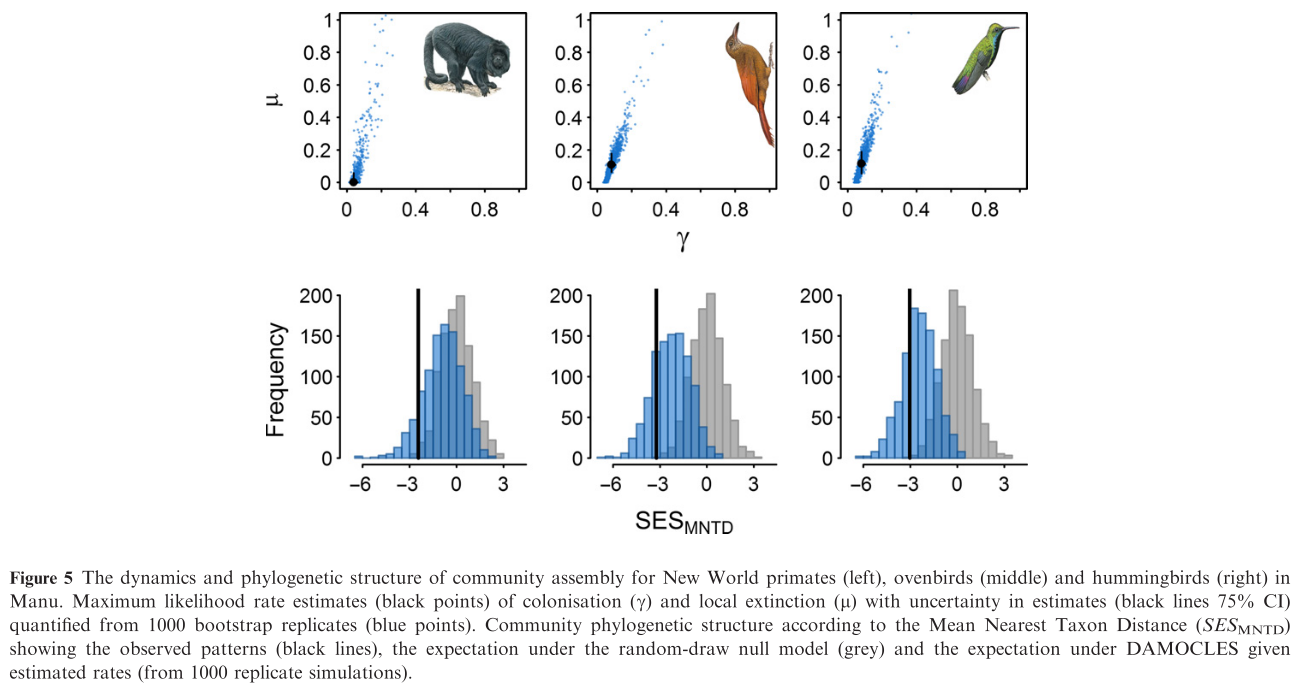
\includegraphics[width=\textwidth]{fig/Pigot2015.png}
%\caption{•}
%\end{figure}
%\vspace{-20pt}
\label{box:Pigot}
\end{bluebox}
\end{figure}

\lipsum[1-3]

\subsection{multicols}

Captions are harder to set in twocolumn environnement, but here is an example. I don't really controle figure in two-columns docs to put them in a reproducible document, but I think time will help with this.

\begin{multicols}{2} 
\lipsum[1-3] 
\end{multicols}

\section{Import other documents}

\subfile{tex/subpart1}

Next is my first master year report, to show examples with figures and all other stuff.

\newpage
\subfile{tex/intro}
\subfile{tex/mat_meth}
\subfile{tex/result}
\subfile{tex/discuss}

%%%%%%%%%%%%%%%%%%%%%%%%%%%%%%%%%%%%%%%%%%%%%%%%%%%%%%%%%%%%%%%%%%%%%%
% Références
%%%%%%%%%%%%%%%%%%%%%%%%%%%%%%%%%%%%%%%%%%%%%%%%%%%%%%%%%%%%%%%%%%%%%%
\newpage
%\subsection*{Bibliographie}
\imp[change bibliography model]
\ifthenelse{\boolean{bib_basic}}{
	\bibliographystyle{authordate1}
}{
	\bibliographystyle{.temp/bst/tree}
%	\bibliographystyle{.temp/bst/mee}
}

\bibliography{Primula}

\begin{web}[h]
	\caption{\url{ https://github.com}}
	\label{igp}
\end{web}

%%%%%%%%%%%%%%%%%%%%%%%%%%%%%%%%%%%%%%%%%%%%%%%%%%%%%%%%%%%%%%%%%%%%%%
% Ressources
%%%%%%%%%%%%%%%%%%%%%%%%%%%%%%%%%%%%%%%%%%%%%%%%%%%%%%%%%%%%%%%%%%%%%%
\subsection*{Ressources}

Ce document est disponible en ligne sous format ``.Rnw'', contenant tout le code néccessaire à la reproduction de l'analyse, réalisée avec un script en langage R \citep{RTeam2017}, ainsi que le jeu de données de départ. L'ensemble est situé sur Github : ~\url{https://github.com/gowachin/Template}

%%%%%%%%%%%%%%%%%%%%%%%%%%%%%%%%%%%%%%%%%%%%%%%%%%%%%%%%%%%%%%%%%%%%%%
% Annexes
%%%%%%%%%%%%%%%%%%%%%%%%%%%%%%%%%%%%%%%%%%%%%%%%%%%%%%%%%%%%%%%%%%%%%%
\subfile{tex/annexes}

%%%%%%%%%%%%%%%%%%%%%%%%%%%%%%%%%%%%%%%%%%%%%%%%%%%%%%%%%%%%%%%%%%%%%%
% word count
\ifthenelse{\boolean{terminal}}{
	\newpage
	\imp[Remove word counts]
	\ifthenelse{\boolean{counter}}{
		\subsubsection*{Counts of words}
		\wordcount
	}{}
}{}

\end{document}


